\documentclass{article}
\usepackage[utf8]{inputenc}

\title{Informe redes de datos: Rutas de redes}
\author{Patricio Inostroza y Matias Castro }
\date{Junio 2017}

\usepackage{natbib}
\usepackage{graphicx}

\begin{document}

\begin{titlepage}

\maketitle
\huge


\end{titlepage}

\tableofcontents 
\cleardoublepage

\section{Introducción}
En el presente informe se verá y analizará el funcionamiento de protocolos de ruteo dinamico y su comportamiento virtual en Packet Tracer, especificamente de EIGRP y OSPF (Enhanced Interior Gateway Routing Protocol-Open Shortest Path First). Para llevar a cabo esto se aprenderá la configuración de los comandos necesarios de los protocolos a través de diferentes topologias, asi mostrar diferencias. Finalmente se responderán preguntas que surgen dado lo que se verá en este informe.


\section{Desarrollo}
 
Para llevar acabo el siguiente procedimiento de ruteo, se necesita acceso al programa Packet Tracer y configurar la siguiente topología (Figura 1) que es entre routers, los comandos que se utilizan son para la configuración EIGRP de ruteo, esto se hace entre routers, como lo vemos en la figura 2, la ip y la máscara de las distintas conexiones, una ip distinta para cada conjunto de routers. 

\begin{figure}[h!]
\centering
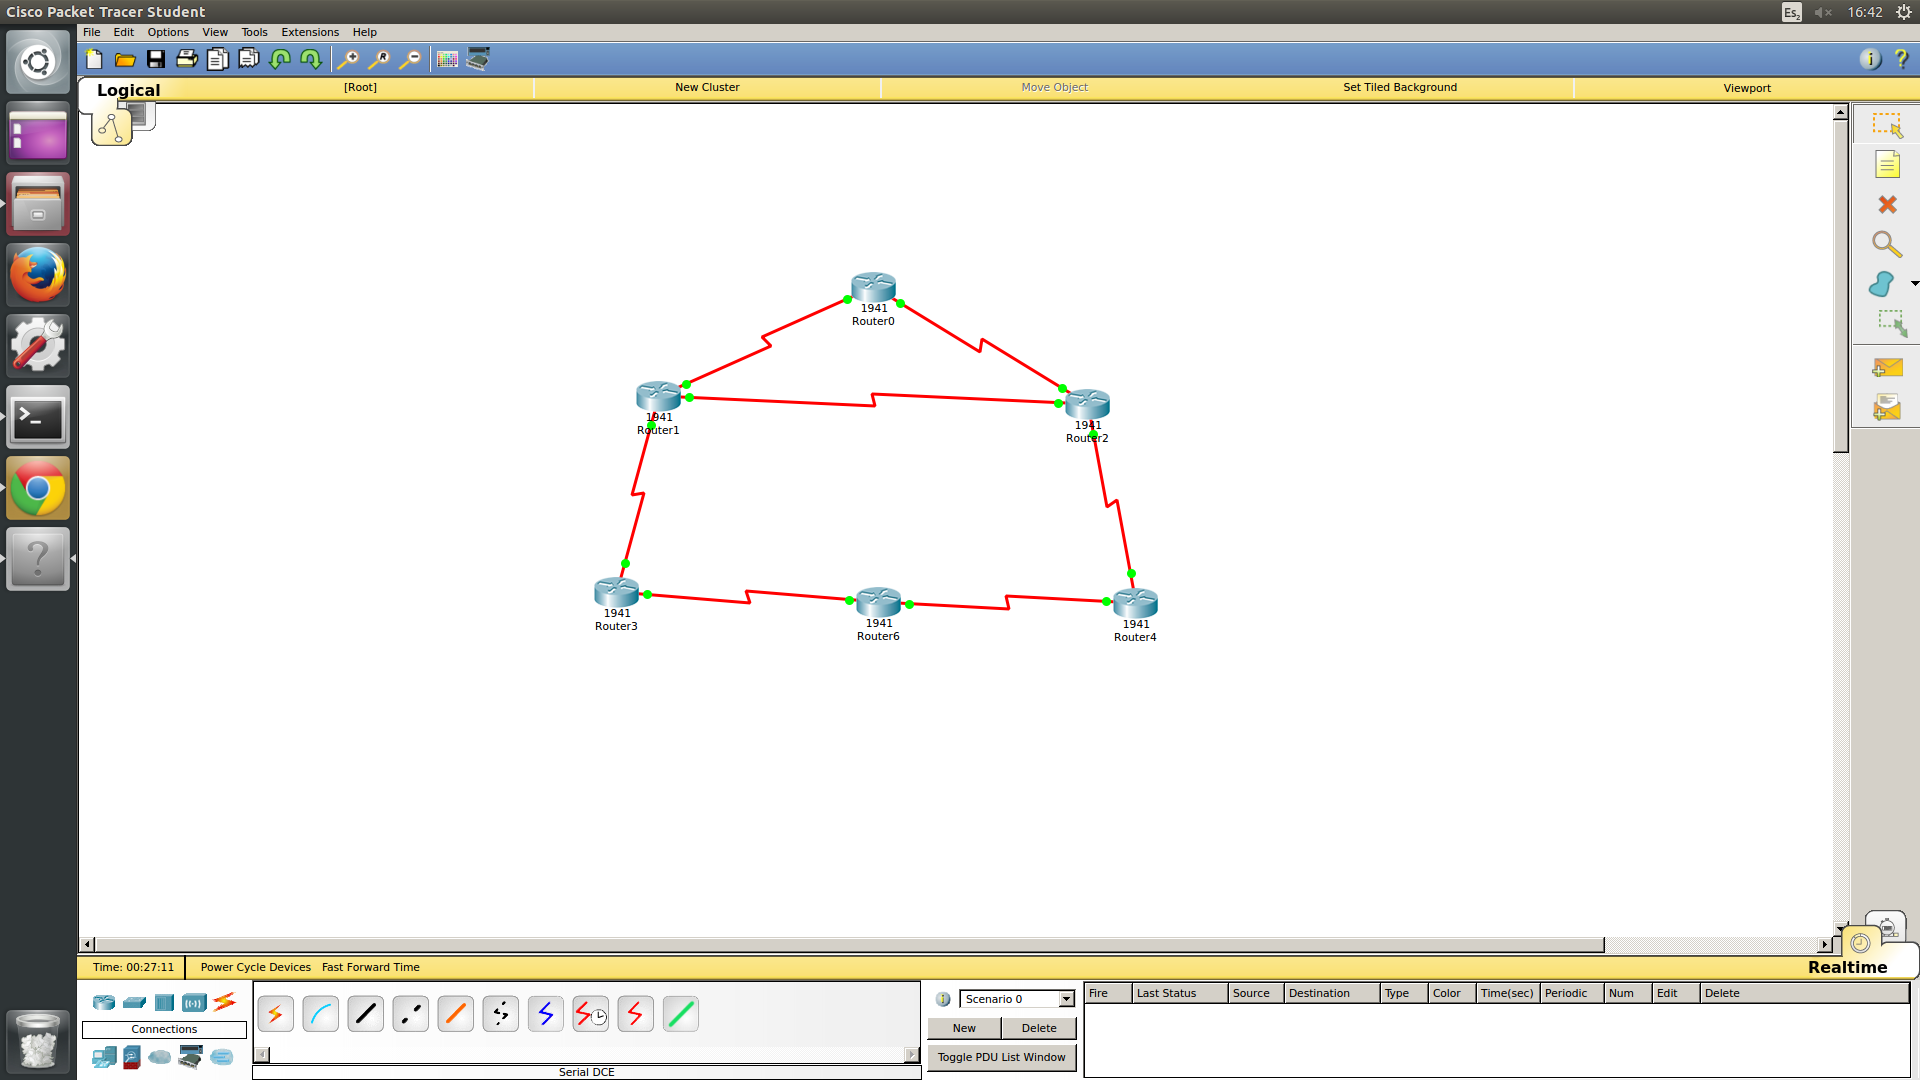
\includegraphics[scale=0.08]{IMG1}
\caption{Topología}
\end{figure}

\begin{figure}[h!]
\centering
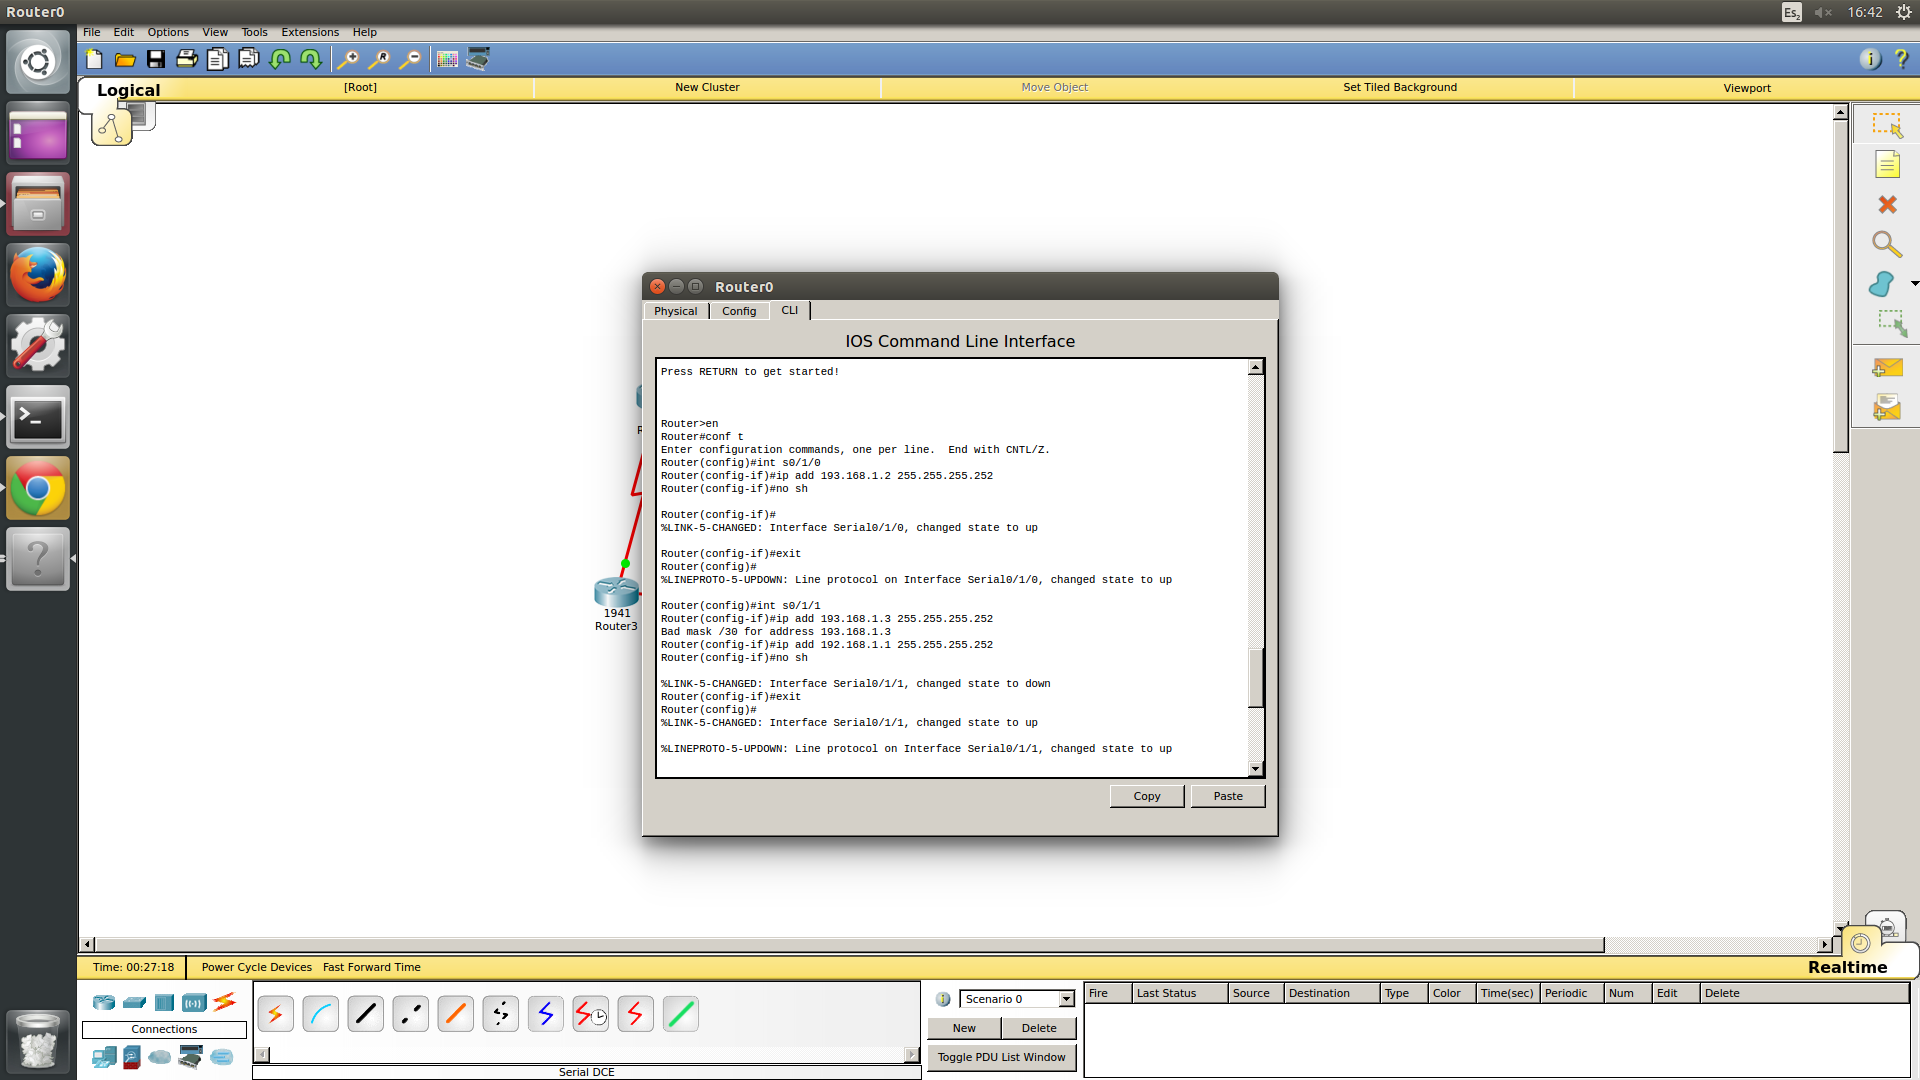
\includegraphics[scale=0.08]{IMG2}
\caption{Comando}
\end{figure}

\newpage

Luego de esto se procede a configurar con los mismos comandos para la LAN de cada router (la conexión al pc, o host), o sea sus puertos fast ethernet. Para esto a la topologia ya creada agregamos un host en cada router, así creamos una LAN. (Figura 3)


Finalmente configuramos nuestro protocolo de enrutamiento dinámico EIGRP que a diferencia de su predecesor funciona con enrutamiento sin clase o con clase (Eltallerdelbit, 2011), siendo un protocolo de transporte que crea tablas para su entorno (sus vecinos, para entenderlo didácticamente). La configuración es como se muestra a continuación en la figura 4: 

\begin{figure}[h!]
\centering
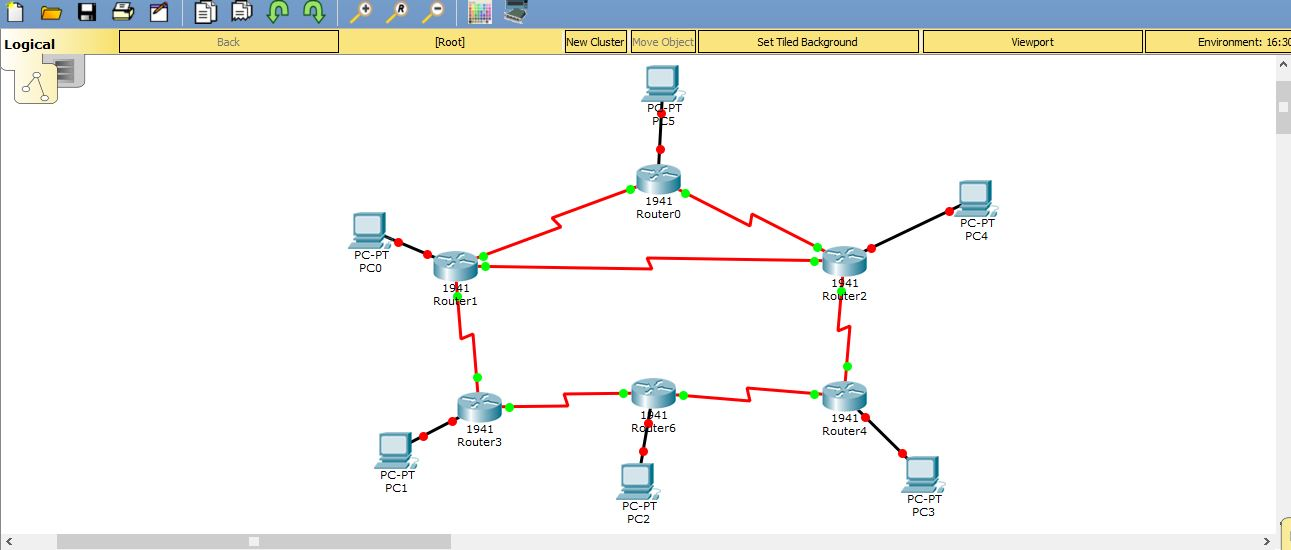
\includegraphics[scale=0.3]{IMG3}
\caption{Topología}
\end{figure}

\begin{figure}[h!]
\centering
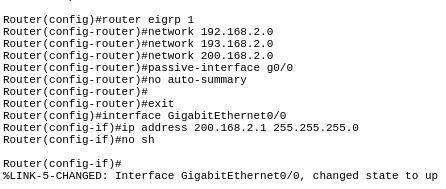
\includegraphics[scale=1]{IMG4}
\caption{Protocolo EIGRP}
\end{figure}


\newpage

\section{Preguntas}
1.-¿Como funciona OSPF?
El Protocolo OSPF (Open Shortest Path First) es un mecanismo que define la ruta a utilizar  usando el algoritmo de Dijkstra; a cada tramo se le asigna un coste y el camino que posea el menor coste es el utilizado.

2.-¿Como funciona el algoritmo de Dijkstra?
El algoritmo de Dijkstra determina el camino mas corto calculando el valor de cada ruta, a cada punto se le otorga una etiqueta y gracias a esa etiqueta que contiene el costo y distancia del nodo anterior.

3.-¿Qué considera mejor; Vector - Distancia o Estado de Enlace?
El Estado de enlace es un mejor protocolo ya que determina el camino considerando mas variables,posee una mejor deteccion de errores, evita loops y es mas rápida.

4.-¿Qué es y como funciona IGRP?
IGRP es un protocolo de enrutamiento Vector-Distancia pero a diferencia del resto, también considera variables del estado del enlace, fue creado por Cisco y posee una versión mejorada: EIGRP


\newpage

\section{Conclusion}
A lo largo del presente informe analizamos el funcionamiento de protocolos de ruteo, cómo reaccionan a los cambios topológicos, cómo son configurados y administrados para que sean mas fáciles en ambos sentidos, cómo tambien OSPF se beneficia al ser un protocolo de estado de enlace, ya que conoce toda la red, contra EIRPG que al ser vector de distancia conoce solamente a su entorno, pero a la vez esto mismo hace que el primero sea mas lento al tener mucha mas información que el ultimo, hay mas opciones para ayudar a OSPF con esto, pero debe ser debidamente pensado y manejado despues, finalmente queda a gusto y facilidad del que ocupe los diferentes protocolos recien mencionados sabiendo en que aspectos tienen desventajas y tambien conociendo sus beneficios.

\newpage

\section{Bibliografia}

Cisco . (Agosto de 2005). Cisco Networking Acedemy. Obtenido de http://www.cisco.com/c/en/us/

support/docs/ip/enhanced-interior-gateway-routing-protocol-eigrp/13669-1.html
El taller del bit. (Noviembre de 2011). El taller del bit. Obtenido de http://eltallerdelbit.com/eigrp

\end{document}
